%% bare_jrnl.tex
%% V1.4b
%% 2015/08/26
%% by Michael Shell
%% see http://www.michaelshell.org/
%% for current contact information.
%%
%% This is a skeleton file demonstrating the use of IEEEtran.cls
%% (requires IEEEtran.cls version 1.8b or later) with an IEEE
%% journal paper.
%%

\documentclass[journal,onecolumn]{IEEEtran}
%
% If IEEEtran.cls has not been installed into the LaTeX system files,
% manually specify the path to it like:
% \documentclass[journal]{../sty/IEEEtran}

\usepackage[pdftex]{graphicx}
\usepackage{amsmath,amssymb,amsfonts,amsthm}
\usepackage{algpseudocode}
\usepackage{algorithm}
\usepackage{xpatch}
\usepackage{cite}
\usepackage{tikz}
\usetikzlibrary{shapes, arrows}

\ifCLASSOPTIONcompsoc
\usepackage[caption=false, font=normalsize, labelfont=sf, textfont=sf]{subfig}
\else
\usepackage[caption=false, font=footnotesize]{subfig}
\fi

\newtheorem{lemma}{Lemma}
\renewcommand{\IEEEQED}{\IEEEQEDclosed}

%\usepackage{array}
%\usepackage[caption=false,font=normalsize,labelfont=sf,textfont=sf]{subfig}
%\usepackage{url}

\hyphenation{op-tical net-works semi-conduc-tor}

%% For algorithms...
\algrenewcommand\alglinenumber[1]{{\sffamily\footnotesize#1:}}
\makeatletter
\xpatchcmd{\algorithmic}{\itemsep\z@}{\itemsep=5pt}{}{}
\makeatother
\renewcommand{\algorithmicrequire}{\textbf{Input:}}
\renewcommand{\algorithmicensure}{\textbf{Output:}}
\renewcommand{\algorithmicforall}{\textbf{For Each}}

% Define block styles for tikz...
\tikzstyle{decision} = [diamond, draw, fill=blue!20, text width=4.5em, 
    text centered, node distance=3cm, inner sep=0pt]
\tikzstyle{block} = [rectangle, draw, fill=blue!20, text width=3cm, 
    text centered, rounded corners, minimum height=4em]
\tikzstyle{info} = [rectangle, scale=0.9, text width=5cm, minimum height=4em, node distance=4.75cm]
\tikzstyle{line} = [draw, -latex']
\tikzstyle{cloud} = [draw, ellipse,fill=red!20, node distance=3cm,
    minimum height=2em]
\tikzstyle{io} = [trapezium, trapezium left angle=70, trapezium right angle=110, 
    minimum height=1cm, text centered, draw=black, fill=blue!30]

\begin{document}
% \title{_}
% \author{_}
% 
% \maketitle

\section{Introduction}
Technological advances in the past few decades have triggered an explosion in the collection of spatio-temporal data.  The increasing popularity of GPS devices and smartphones, along with the emergence of new disciplines such as the Internet of Things (IoT) and high-resolution Satellite/UAS imagery, has made it possible to collect vast amounts of data with spatial and temporal components.

In tandem, interest in extracting valuable information from such large databases has also grown.  Spatio-temporal queries about popular places or frequent events remain useful, but there has been growing interest in more complex patterns.  In particular, patterns that describe the group behavior of moving objects over significant periods.  Moving cluster \cite{kalnis_discovering_2005}, convoys \cite{jeung_discovery_2008}, flocks \cite{gudmundsson_computing_2006} and swarm patterns \cite{li_swarm_2010} reveal how entities move together over a minimum time interval.

Applications for this type of information are both diverse and intriguing, particularly when dealing with trajectory datasets \cite{jeung_trajectory_2011, huang_mining_2015}. Case studies span various domains, including transportation system management and urban planning \cite{di_lorenzo_allaboard_2016}, as well as ecology \cite{la_sorte_convergence_2016}. For example, \cite{turdukulov_visual_2014} explores the identification of complex motion patterns to discover similarities in tropical cyclone paths. Similarly, \cite{amor_persistence_2016} investigates eye movement trajectories to understand the strategies people use during visual searches. Additionally, \cite{holland_movements_1999} tracks the behavior of tiger sharks along the coasts of Hawaii to gain insight into their migration patterns.

One particular pattern of interest is the moving flock pattern, which captures how objects move within close proximity for a given time period. Closeness is defined by a disk of a specified radius within which the entities must remain. Since this disk can be positioned anywhere, detecting such patterns is a non-trivial problem. In fact, \cite{gudmundsson_computing_2006} highlights that finding flock patterns where the same entities stay together over time is an NP-hard problem. To address this, \cite{vieira_2009} proposed the BFE algorithm, the first approach capable of detecting flock patterns in polynomial time.

Despite the increasing availability of data, current state-of-the-art techniques for mining complex movement patterns still struggle with the performance demands of large-scale spatial data. This work introduces a scalable approach designed to detect moving flock patterns in very large trajectory databases. By leveraging emerging trends in distributed frameworks for spatial operations we aim to significantly improve the speed and efficiency of detecting these patterns.

\section{Related work}
The recent increased use of location-aware devices (such as GPS, smartphones, and RFID tags) has enabled the collection of vast amounts of data with spatial and temporal components.  Several studies have focused on discovering and analyzing these types of datasets \cite{leung_knowledge_2010, miller_geographic_2001}.  In this area, trajectory datasets have emerged as an interesting field where diverse kind of patterns can be identified \cite{zheng_computing_2011, vieira_spatio-temporal_2013}.  For instance, researchers have proposed techniques to discover spatial motion patterns such as moving clusters \cite{kalnis_discovering_2005}, convoys \cite{jeung_discovery_2008} and flocks \cite{benkert_reporting_2008, gudmundsson_computing_2006}.  Specifically, \cite{vieira_2009} introduced BFE (Basic Flock Evaluation), an innovative algorithm designed to efficiently identify moving flock patterns in polynomial time across large spatio-temporal datasets.

A flock pattern is defined as a group of entities that move together over a specified time period \cite{benkert_reporting_2008}. The applications of such patterns are broad and diverse. For instance, \cite{calderon_romero_mining_2011} identifies moving flock patterns in iceberg trajectories to analyze their movement behavior and their relationship with changes in ocean currents.

The BFE algorithm provides an initial approach for detecting flock patterns. It begins by identifying disks with a predefined diameter ($\varepsilon$) where moving entities are sufficiently close at specific time instants. This operation is computationally expensive due to the large number of points and time instances to be analyzed, with a complexity of $\mathcal{O}(2n^2)$ per time. Although the algorithm leverages a grid-based index and a stencil to accelerate this process, the overall complexity remains high.

Both \cite{calderon_romero_mining_2011} and \cite{turdukulov_visual_2014} adopt a frequent pattern mining approach to enhance performance when combining disks across time instants. Similarly, \cite{tanaka_improved_2016} utilize plane sweeping techniques, binary signatures, and inverted indexes to further accelerate this process. However, these methods retain the core strategy of BFE for detecting disks at each time instant.

In contrast, \cite{arimura_finding_2014} and \cite{geng_enumeration_2014} employ depth-first algorithms to analyze the time intervals of individual trajectories and report maximal duration flocks. However, these methods are less effective for dense datasets or those that involve large numbers of entities per time step, as they struggle to scale efficiently in such conditions.

Given the high computational demands of flock pattern detection, it is not surprising that parallelism has been employed to improve performance. For example, \cite{fort_parallel_2014} use extreme and intersection sets to report maximal, longest, and largest flocks on GPUs, albeit with limitations imposed by the GPU's memory model.

Despite the increasing adoption of cluster computing frameworks, particularly those with spatial data capabilities \cite{eldawy_spatialhadoop_2014, yu_demonstration_2016, pellechia_geomesa_2015, xie_simba_2016}, significant advancements in this area remain limited. To the best of our knowledge, this work is the first to explore the detection of moving flock patterns in a scalable approach.

\section{Scalable Kd-tree Partitioner with Dangle and Cut Edges Integration} \label{sec:extension_methods}

\subsubsection{Kd-tree Partition Strategy} %\label{sec:kdtreestrategy}
In Section \ref{sec:pstrategies}, we use the quadtree spatial index as the baseline for our partitioning strategy. The quadtree follows a space-oriented approach, as it does not consider the content of each cell when determining potential splits. In contrast, kd-tree-based partitioning employs a data-oriented approach by sorting and selecting the midpoint within a cell to guide the placement of splits for future child nodes.

Building and populating the kd-tree partitioning follows a process similar to that of the quadtree. First, a kd-tree is constructed from a sample representing 1\% of the input data to define the tree’s structure, where the leaves represent the partition’s cells. The input data is then fed into this kd-tree structure, with each edge assigned to the leaf cell containing its boundaries. After partitioning, the local DCELs for each layer are constructed, and the overlay operation is performed within each cell as described in Section \ref{sec:pstrategies}.

Section \ref{sec:extension_experiments} will compare two partitioning strategies, the one presented in \ref{sec:pstrategies} based on the quadtree (i.e. space-oriented) and one on the kd-tree (i.e. data-oriented) indexes.  Note that both tree-based data partitioning involves shuffling all edges; this however, happens only once. Our experimental evaluation (see Section \ref{sec:comparison}) shows that the data-oriented approach leads to better performance. 

\subsection{Overlaying Polygons with Dangle and Cut Edges} \label{sec:over_dang}

Beyond scalability challenges, many modern applications receive spatial polygon datasets as scattered line segments—for example, road segments that form city blocks. Such datasets can be extremely large and are common in fields like urban planning, geo-targeted advertising, economic and demographic studies, and more. However, existing polygon overlay techniques are not equipped to process them directly at scale. In this section, we extend the overlay method presented in Section \ref{sec:methods} to support polygonal input by integrating a scalable, distributed polygon extraction approach. This enhancement enables the merging of polygons with dangle and cut edges.

We built on in the scalable polygonization procedure presented in \cite{abdelhafeez_ddcel_2023}.  The result of that polygonization procedure generates two outputs: first, a set of closed polygons formed by the input planar line segments, and second, any edges that are not a part of any polygon (i.e., dangle or cut edges).  Overlaying the polygons generated with any polygon layer follows the approaches discussed in sections \ref{sec:methods} and \ref{sec:alternative_methods}.  However, we need to modify the algorithms provided in these previous sections to overlay an input polygon layer $A$ with the dangle and cut edges (layer $B$). In particular, we modify the reduce phase.

We build upon the scalable polygonization procedure presented in \cite{abdelhafeez_ddcel_2023} (see Figure \ref{fig:polygonization}), which produces two outputs: (1) a set of closed polygons formed from the input planar line segments, and (2) any edges that are not part of any polygon (i.e., dangle or cut edges). Overlaying these generated polygons with any polygon layer follows the methods discussed in Sections \ref{sec:methods} and \ref{sec:alternative_methods}. However, to overlay an input polygon layer $A$ with the dangle and cut edges (layer $B$), we modify the algorithms from these sections, particularly adjusting the reduce phase.

 \begin{figure}
     \centering
     \begin{tabular}{cc}
         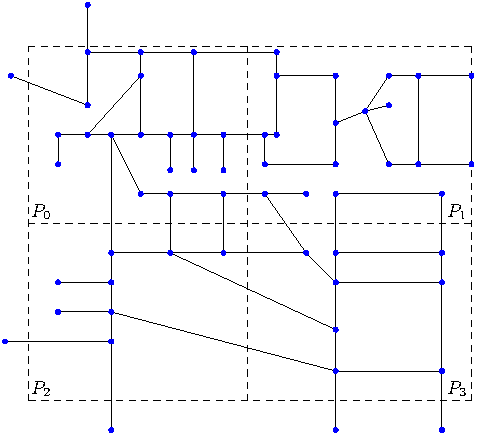
\includegraphics[width=0.49\textwidth]{chapterExtension/model/input/input} &
         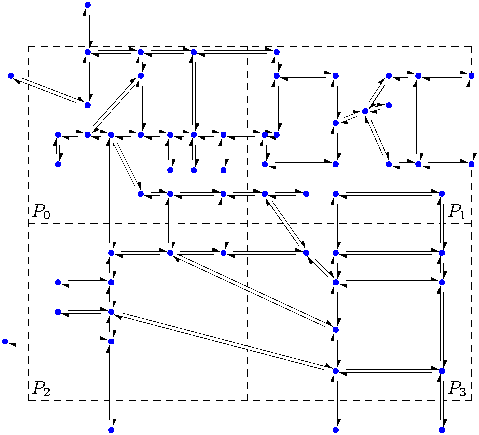
\includegraphics[width=0.49\textwidth]{chapterExtension/model/a/a} \\
         (a) & (b) \\
         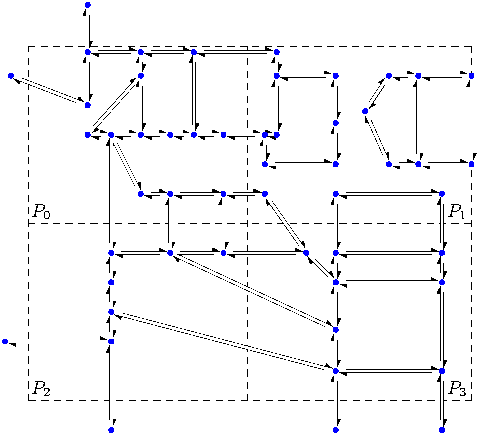
\includegraphics[width=0.49\textwidth]{chapterExtension/model/b/b} &
         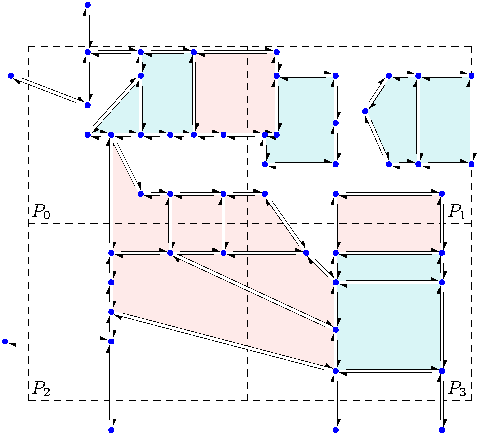
\includegraphics[width=0.49\textwidth]{chapterExtension/model/c/c} \\
         (c) & (d) \\
     \end{tabular}
     \caption{An example of four leaf nodes in a quadtree constructed for input spatial line segments. Solid lines represent the line segments, while dashed lines indicate the Minimum Bounding Rectangles (MBRs) of the partitions. (a) shows the partitioned input spatial lines. (b) shows the DCEL vertices and half-edges. (c) the resulting DCEL after  dangle and cut edge removal.  Finally, (d) shows the final DCEL faces. (taken from \cite{abdelhafeez_ddcel_2023}).} \label{fig:polygonization}
 \end{figure}

 \begin{figure}
    \centering
    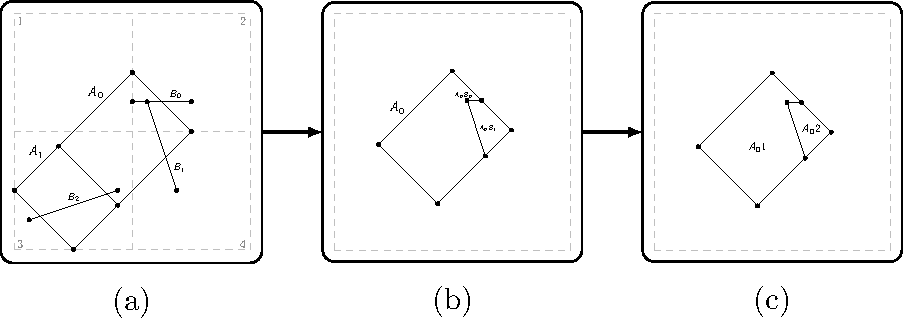
\includegraphics[width=\textwidth]{chapterExtension/dangles_cuts/DAC}
    \caption{(a) Spatial partitioning of input layers A and B, (b) Re-Partitioning of polygon $A_0$ with edges it intersects with, and (c) the result of polygonization of $A_0$ with $B_0, B_1, B_2$.} \label{fig:dangles_cuts}
 \end{figure}

 Figure \ref{fig:dangles_cuts}(a) illustrates the spatial partitioning of two input layers, $A$ and $B$. Layer $A$ contains two input polygons, $A_0$ and $A_1$, while Layer $B$ includes of three dangle edges, $B_0$, $B_1$, and $B_2$.
 
 Each edge in layer $B$ is assigned a unique label and provided as input to the overlay module.  The local overlay processs indentifies intersections between the input polygon layer $A$ and layer $B$ within each data partition.  If a polygon with $id = i$ from layer $A$ intersects with edges labeled $id = a$, $id = b$ and $id = c$ from layer $B$ in a given partition, a composite label $A_{i} B_{a} B_{b} B_{c}$ is generated to represent these intersections.  
 
During the reduce phase, we re-partition the data based on the first label, consolidating all edges that intersect with it. For instance, if two data partitions generate the labels $A_{i} B_{a} B_{b} B_{c}$ and $A_{i} B_{x} B_{y}$, we reassign the data so that $A_{i}$ is grouped within a single partition along with all intersecting edges, specifically $B_{a}, B_{b}, B_{c}, B_{x}, B_{y}$.  In Figure \ref{fig:dangles_cuts}(b), polygon $A_0$ is re-partitioned with the edges it intersects, namely $B_0$, $B_1$, and $B_2$.

After re-partitioning, all intersecting edges from both layers are consolidated within the same partition. The next step is to identify the polygons formed by these intersections. Since there is no guarantee that only one polygon will be generated, we replace the polygon concatenation method proposed in Section \ref{sec:optimizing} with a \textit{polygonization} procedure within each partition. This polygonization process ensures that all possible new polygons are generated.

The polygonization procedure follows the algorithm outlined in \cite{abdelhafeez_ddcel_2023}. It begins by generating new vertices and half-edges, marking the current dangle and cut edges, setting the next pointers, and finally constructing the partition polygons. Figure \ref{fig:dangles_cuts}(c) illustrates the result of polygonizing the edges from polygon$A_0$ and $B_0$, $B_1$, and $B_2$, yielding two polygons,$A_01$ and $A_02$.  The polygons generated from all partitions together form the overlay between polygon layer $A$ and layer $B$.


\bibliographystyle{IEEEtran}
\bibliography{pflocks.bib}
\newpage 
\appendix

\section{Center computation.}
\begin{algorithm}
    \caption{Find the centers of given radius which circumference laid on the two input points.}
    \begin{algorithmic}[1]
        \Require Radius $\frac{\varepsilon}{2}$ and points $p_1$ and $p_2$.
        \Ensure Centers $c_1$ and $c_2$.
        
        \Function{FindCenters}{$p_1$, $p_2$, $\frac{\varepsilon}{2}$}
        \State $r^2 \gets (\frac{\varepsilon}{2})^2$
        \State $X \gets p_1.x - p_2.x$
        \State $Y \gets p_1.y - p_2.y$
        \State $d^2 \gets X^2 + Y^2$
        \State $R \gets \sqrt{\lvert 4 \times \frac{r^2}{d^2} - 1 \rvert}$
        \State $c_1.x \gets X + \frac{Y \times R}{2} + p_2.x$
        \State $c_1.y \gets Y - \frac{X \times R}{2} + p_2.y$
        \State $c_2.x \gets X - \frac{Y \times R}{2} + p_2.x$
        \State $c_2.y \gets Y + \frac{X \times R}{2} + p_2.y$
        
        \State \Return $c_1$ and $c_2$
        \EndFunction
    \end{algorithmic}
    \label{app:centers}
\end{algorithm}

\section{Disk pruning.}
\begin{algorithm}
    \caption{Prune disks which are duplicate or subset of others.}
    \begin{algorithmic}[1]
        \Require Set of disks $D$.
        \Ensure Set of disks $D^{\prime}$ without duplicate or subsets.
        
        \Function{PruneDisks}{$D$}
        \State $E \gets \varnothing$
        \ForAll{disk $d_i$ in $D$}
            \State $N \gets d_i \cap D$
            \ForAll{disk $n_j$ in $N$}
                \If{$d_i$ contains all the elements of $n_j$}
                        \State $E \gets E \cup {n_j}$
                \EndIf
            \EndFor
        \EndFor        
        \State $D^{\prime} \gets D \setminus E$
        \State \Return $D^{\prime}$
        \EndFunction
    \end{algorithmic}
    \label{app:disks}
\end{algorithm}

\section{Clique and MBC approach.}
\begin{figure}
    \centering
    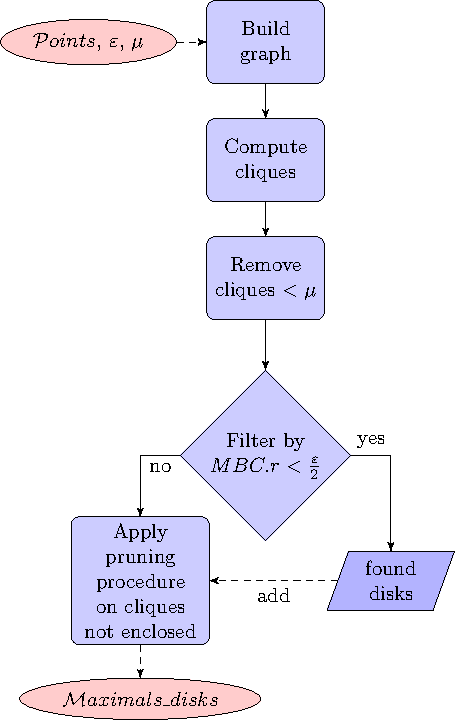
\includegraphics[width=0.7\linewidth]{figures/plots/10_cmbc_variants/CMBC_flowchart2.pdf}
    \caption{Schematic description of the Clique and MBC approach.}
    \label{fig:cmbc_flowchart}
\end{figure}

\end{document}
